\documentclass[aspectratio=169,11pt]{beamer}

\usetheme{Madrid}
\usecolortheme{default}

\usepackage[T1]{fontenc}
\usepackage{lmodern}
\usepackage{tikz}
\usetikzlibrary{positioning}
\usepackage{hyperref}

\definecolor{mainblue}{RGB}{38, 84, 124}
\definecolor{softblue}{RGB}{230, 241, 250}
\definecolor{softgreen}{RGB}{231, 247, 238}
\definecolor{softorange}{RGB}{255, 242, 224}
\definecolor{darkgray}{RGB}{55, 65, 81}

\setbeamercolor{structure}{fg=mainblue}
\setbeamercolor{frametitle}{fg=white,bg=mainblue}
\setbeamercolor{title}{fg=white,bg=mainblue}
\setbeamertemplate{navigation symbols}{}

\title{Python Library Skeleton}
\subtitle{Project Log for the R-to-Python Port}
\author{Rares Calin Olteanu}
\date{\today}

\newcommand{\folderbox}[3]{%
  \node[
    draw=#1,
    fill=#2,
    rounded corners=3pt,
    minimum width=4.1cm,
    minimum height=0.75cm,
    align=center,
    font=\small
  ] (#3) {#3};
}

\begin{document}

\begin{frame}
  \titlepage
\end{frame}

\begin{frame}{Step 1: Main Project Folder}
  \centering
  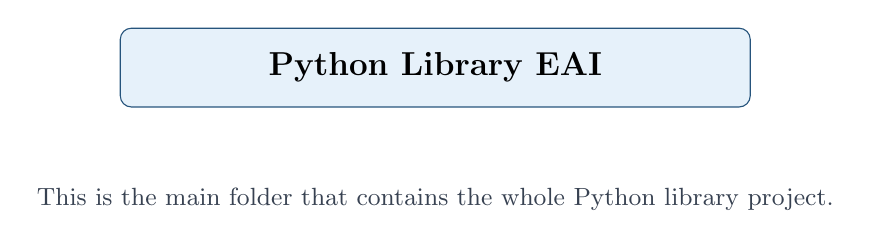
\begin{tikzpicture}[node distance=1.1cm]
    \node[
      draw=mainblue,
      fill=softblue,
      rounded corners=4pt,
      minimum width=8cm,
      minimum height=1cm,
      font=\large\bfseries
    ] (root) {Python Library EAI};

    \pause
    \node[
      below=0.9cm of root,
      align=center,
      text=darkgray,
      font=\small
    ] {This is the main folder that contains the whole Python library project.};
  \end{tikzpicture}
\end{frame}

\begin{frame}{Step 2: Package Metadata}
  \centering
  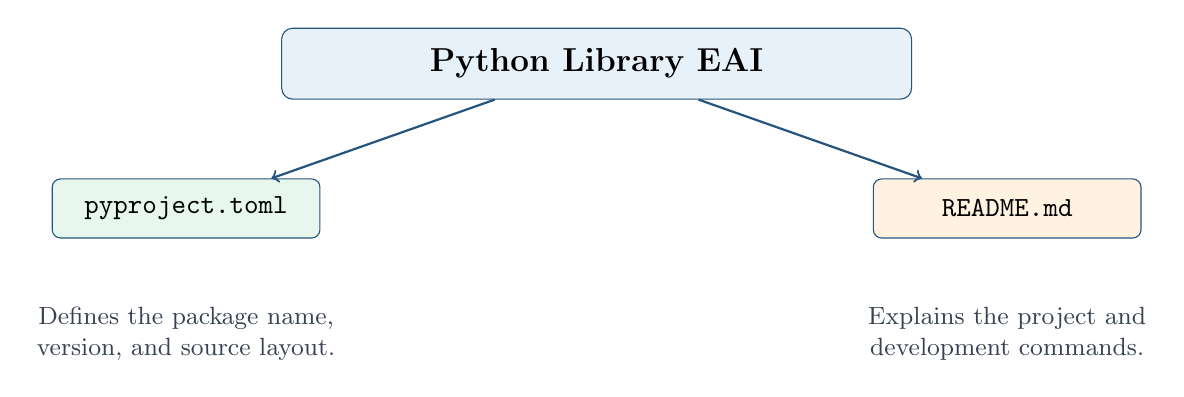
\begin{tikzpicture}[node distance=1.05cm]
    \node[
      draw=mainblue,
      fill=softblue,
      rounded corners=4pt,
      minimum width=8cm,
      minimum height=0.9cm,
      font=\large\bfseries
    ] (root) {Python Library EAI};

    \pause
    \node[
      draw=mainblue,
      fill=softgreen,
      rounded corners=3pt,
      below left=1cm and -0.5cm of root,
      minimum width=3.4cm,
      minimum height=0.75cm
    ] (pyproject) {\texttt{pyproject.toml}};

    \node[
      draw=mainblue,
      fill=softorange,
      rounded corners=3pt,
      below right=1cm and -0.5cm of root,
      minimum width=3.4cm,
      minimum height=0.75cm
    ] (readme) {\texttt{README.md}};

    \draw[->, thick, mainblue] (root) -- (pyproject);
    \draw[->, thick, mainblue] (root) -- (readme);

    \pause
    \node[below=0.75cm of pyproject, align=center, font=\small, text=darkgray] {
      Defines the package name,\\ version, and source layout.
    };

    \node[below=0.75cm of readme, align=center, font=\small, text=darkgray] {
      Explains the project and\\ development commands.
    };
  \end{tikzpicture}
\end{frame}

\begin{frame}{Step 3: Source Code Folder}
  \centering
  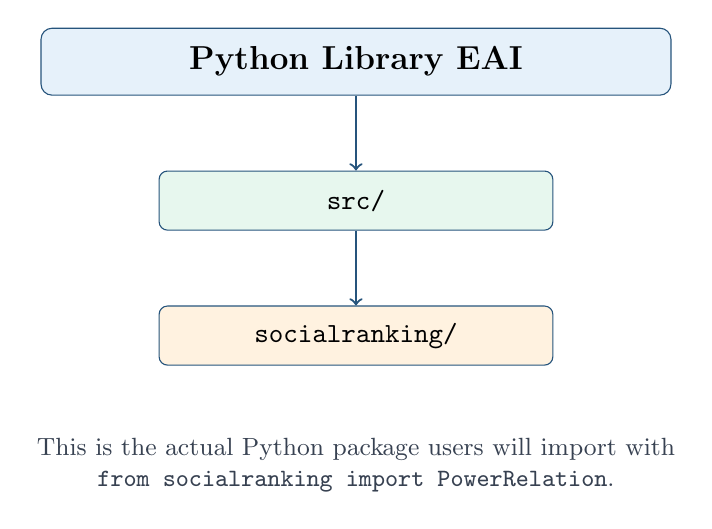
\begin{tikzpicture}[node distance=1.05cm]
    \node[
      draw=mainblue,
      fill=softblue,
      rounded corners=4pt,
      minimum width=8cm,
      minimum height=0.85cm,
      font=\large\bfseries
    ] (root) {Python Library EAI};

    \pause
    \node[
      draw=mainblue,
      fill=softgreen,
      rounded corners=3pt,
      below=0.95cm of root,
      minimum width=5cm,
      minimum height=0.75cm
    ] (src) {\texttt{src/}};
    \draw[->, thick, mainblue] (root) -- (src);

    \pause
    \node[
      draw=mainblue,
      fill=softorange,
      rounded corners=3pt,
      below=0.95cm of src,
      minimum width=5cm,
      minimum height=0.75cm
    ] (pkg) {\texttt{socialranking/}};
    \draw[->, thick, mainblue] (src) -- (pkg);

    \pause
    \node[below=0.8cm of pkg, align=center, font=\small, text=darkgray] {
      This is the actual Python package users will import with\\
      \texttt{from socialranking import PowerRelation}.
    };
  \end{tikzpicture}
\end{frame}

\begin{frame}{Step 4: Library Files}
  \centering
  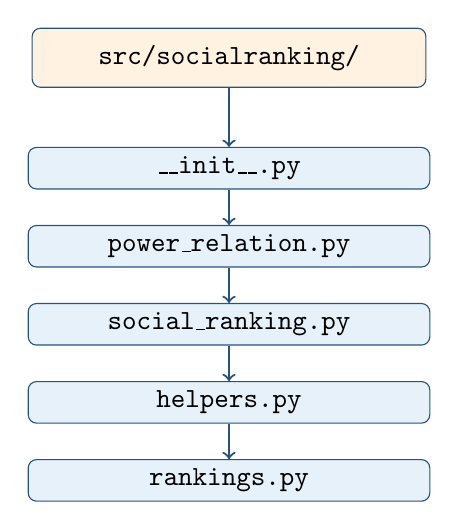
\begin{tikzpicture}[node distance=0.6cm]
    \node[
      draw=mainblue,
      fill=softorange,
      rounded corners=3pt,
      minimum width=5cm,
      minimum height=0.75cm,
      font=\bfseries
    ] (pkg) {\texttt{src/socialranking/}};

    \pause
    \node[draw=mainblue, fill=softblue, rounded corners=3pt, below=0.75cm of pkg, minimum width=5.1cm] (init) {\texttt{\_\_init\_\_.py}};
    \pause
    \node[draw=mainblue, fill=softblue, rounded corners=3pt, below=0.45cm of init, minimum width=5.1cm] (pr) {\texttt{power\_relation.py}};
    \pause
    \node[draw=mainblue, fill=softblue, rounded corners=3pt, below=0.45cm of pr, minimum width=5.1cm] (sr) {\texttt{social\_ranking.py}};
    \pause
    \node[draw=mainblue, fill=softblue, rounded corners=3pt, below=0.45cm of sr, minimum width=5.1cm] (helpers) {\texttt{helpers.py}};
    \pause
    \node[draw=mainblue, fill=softblue, rounded corners=3pt, below=0.45cm of helpers, minimum width=5.1cm] (rankings) {\texttt{rankings.py}};

    \draw[->, thick, mainblue] (pkg) -- (init);
    \draw[->, thick, mainblue] (init) -- (pr);
    \draw[->, thick, mainblue] (pr) -- (sr);
    \draw[->, thick, mainblue] (sr) -- (helpers);
    \draw[->, thick, mainblue] (helpers) -- (rankings);
  \end{tikzpicture}
\end{frame}

\begin{frame}{Step 5: Tests and R Reference Code}
  \centering
  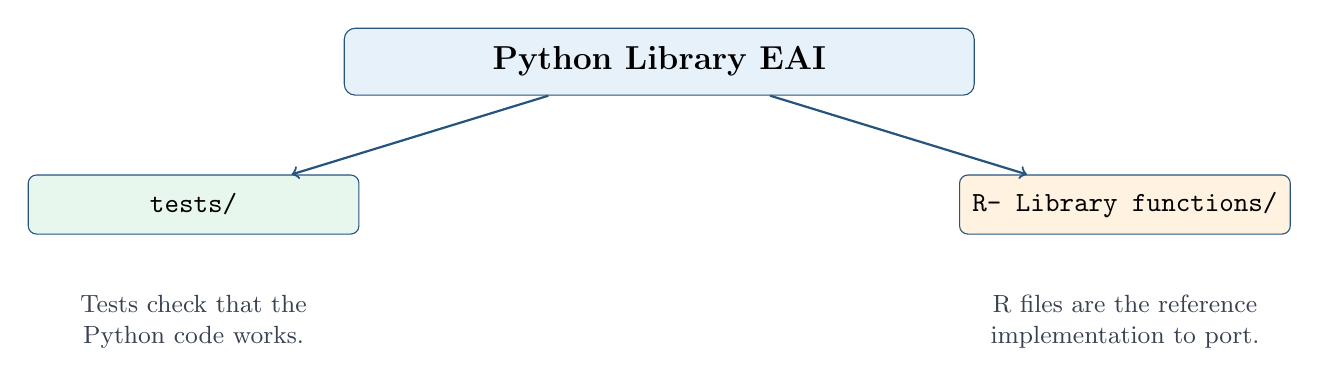
\begin{tikzpicture}[node distance=0.9cm]
    \node[
      draw=mainblue,
      fill=softblue,
      rounded corners=4pt,
      minimum width=8cm,
      minimum height=0.85cm,
      font=\large\bfseries
    ] (root) {Python Library EAI};

    \pause
    \node[
      draw=mainblue,
      fill=softgreen,
      rounded corners=3pt,
      below left=1cm and -0.2cm of root,
      minimum width=4.2cm,
      minimum height=0.75cm
    ] (tests) {\texttt{tests/}};

    \node[
      draw=mainblue,
      fill=softorange,
      rounded corners=3pt,
      below right=1cm and -0.2cm of root,
      minimum width=4.2cm,
      minimum height=0.75cm
    ] (rfiles) {\texttt{R- Library functions/}};

    \draw[->, thick, mainblue] (root) -- (tests);
    \draw[->, thick, mainblue] (root) -- (rfiles);

    \pause
    \node[below=0.65cm of tests, align=center, font=\small, text=darkgray] {
      Tests check that the\\ Python code works.
    };

    \node[below=0.65cm of rfiles, align=center, font=\small, text=darkgray] {
      R files are the reference\\ implementation to port.
    };
  \end{tikzpicture}
\end{frame}

\begin{frame}{Current Skeleton Summary}
  \begin{block}{What exists now}
    \begin{itemize}
      \item A modern Python package structure.
      \item A package named \texttt{socialranking}.
      \item Initial files for \texttt{PowerRelation}, \texttt{SocialRanking}, helpers, and rankings.
      \item A tests folder with basic tests.
    \end{itemize}
  \end{block}

  \pause

  \begin{block}{Next implementation step}
    Properly port \texttt{PowerRelation}, because almost every other R function depends on it.
  \end{block}
\end{frame}

\end{document}
